\documentclass[conference]{IEEEtran}

\usepackage{cite}
\usepackage{amsmath,amssymb,amsfonts}
\usepackage{algorithmic}
\usepackage{graphicx}
\usepackage{textcomp}
\usepackage{xcolor}
%\usepackage{flushend}
\def\BibTeX{{\rm B\kern-.05em{\sc i\kern-.025em b}\kern-.08em
    T\kern-.1667em\lower.7ex\hbox{E}\kern-.125emX}}

\IEEEoverridecommandlockouts
\begin{document}

\title{A Code-First Approach to Teaching Software Design Patterns}

\author{\IEEEauthorblockN{Jeffrey Hemmes}
\IEEEauthorblockA{\textit{Department of Computer and Cyber Sciences} \\
\textit{United States Air Force Academy}\\
jeffrey.hemmes@afacademy.af.edu}
\thanks{\noindent{{The views expressed in this document are those of the authors and do not reflect the official policy or position of the United States Air Force, Department of Defense, or the U.S. Government.}}}}

\maketitle


\begin{abstract}
Software design patterns are a cornerstone of professional software engineering education, yet traditional approaches to teaching them often fail students by leading with abstraction. This paper proposes and evaluates a \emph{code-first, pattern-second} (CFPS) pedagogical framework in which students encounter concrete implementation problems before being introduced to the canonical pattern that resolves them. Drawing on constructivist learning theory, cognitive load theory, and empirical observations from undergraduate software engineering courses, we argue that grounding pattern instruction in executable code produces deeper conceptual transfer, stronger retention, and greater practical confidence than the conventional pattern-then-example sequence. We describe the CFPS instructionalmodel in detail, illustrate it through three representative patterns---Observer, Strategy, and Factory Method---and discuss curriculum design implications for instructors adopting approach.
\end{abstract}

\section{Introduction}
Undergraduate survey courses in software engineering typically include blocks of instruction covering design patterns. The topic is important because it represents an important step beyond simply learning programming language syntax, algorithms, and data structures, and towards development of scalable software-intensive systems that are easier to understand, maintain, and reuse. Software design patterns are an important tool in professional software development to help organize code, manage complexity, and provide flexibility and maintainability, particularly in larger-scale or critical systems. Design patterns also provide a common vocabulary with which software engineers can communicate complex design concepts in an efficient and shorthand manner. They represent solutions to commonly recurring design problems, and recognizing those problems as they appear allow students to work more efficiently by avoiding having to solve problems that previously have already been solved by others.

Teaching design patterns as part of an undergraduate course poses two challenges to course designers and instructors. First, although they represent an important concept to apply in professional practice, the majority of students taking a software engineering course as part of an undergraduate program typically lack programming maturity and experience in software development. Consequently, it is common for students to relate to the types of design problems patterns solve. Commonly, software engineering courses are taken during a student's junior year, or perhaps fall semester of their senior year. By that time, students often have completed only a handful of computer science courses, and most likely have not worked on a larger-scale software development effort. This is almost paradoxical: students need to understand and apply concepts related to professional software development practice, while simultaneously lacking the experience and conceptual knowledge to do so. The all-too-frequent result is that design pattern concepts remain abstract and unrelatable to students, and they do not internalize the material as much as instructors may hope.

The second challenge in teaching design patterns to undergraduate students lies in the nature of the material. Going back to the Gang of Four catalog, design patterns have always been organized in a taxonomy with three primary categories: creational patterns; structural patterns; and behavioral patterns. Each category, then contains a collection of patterns. The most common, traditional approach to teaching design patterns involves presenting them in a dry, methodical manner heavy on lecture and mirroring the structure of the Gang of Four taxonomy. Then, for each pattern, the general design problem is presented, followed by the abstract solution model, and then perhaps lastly some example code in an object-oriented programming language. Beyond the original Gang of Four, catalogs of additional patterns are introduced with some regularity as new problems and associated designs arise, e.g.,~\cite{alahmad2006}.

The latter challenge represents a more significant barrier to the effective teaching of design patterns: doing so is boring, repetitious, and not engaging to students. Despite the importance of the topic, students often have difficulty retaining much of the details and nuances of various patterns and might retain only basic information, such as the nature of a Singleton pattern, for instance. It has long been acknowledged that design patterns are ``both difficult to learn and teach.''~\cite{pillay2010}.

Part of the reason for this difficulty is that we tend to focus on the abstract before the implementation (a significant tenet of object oriented design and programming). However, without the requisite background and maturity in programming, the abstract concepts tend to be difficult to grasp.

What if we flip the script and start with the familiar, then work our way up to new concepts? How can we take a bottom-up approach to teaching design patterns and making it more engaging than a standard lecture?

\section{Related Work}

Despite decades of community experience in teaching software design patterns to undergraduate computer science students, there is a dearth of literature describing pedagogical best practices in this topic area. That is not to say, however, that teaching design patterns is an area of software engineering education that cannot be improved. Given the lack of recent literature, it is unlikely that current teaching of patterns is fully aligned with best practices in student-centered learning techniques. This section provides a brief survey of the literature reflecting current pedagogical practice.

Examining existing code to determine appropriate applications of design patterns is certainly nothing new. Since the introduction of the Gang of Four's Design Patterns catalog~\cite{gamma1994}, patterns have been covered in undergraduate programming courses, even as early as CS1~\cite{wallingford1996}. The benefits of using patterns to create elegant, maintainable software designs similarly has a lengthy history~\cite{schmidt1995}, which is commonly emphasized in lesson materials as motivation.

One common practice is to provide students with an existing program of some size that either contains patterns fully implemented~\cite{chimalakonda2018}, or provides opportunities to apply patterns in code that does not already contain them. Commonly we see this using examples of computer games~\cite{gestwicki2008, healy2023, valdick2026}. These types of programs tend to be rather large with some inherent complexity. Games also tend to be designed and implemented using multiple logical layers representing separation of concerns, e.g., graphics, gameplay, data, etc., and therefore there is an abundance of opportunity for students to discover improvement areas and modify the design and implementation through application of patterns. However, to do so effectively, students must already be familiar with some subset of the catalog of design patterns. But how do they learn that catalog in the first place? Ultimately, even current practice for presenting patterns commonly involves lecturing over the catalog pf patterns, stepping through the the design problem for each pattern, and presening the abstract model, typically using the Unified Modeling Language (UML).



\section{Methodology}

declarative and procedural knowledge

-------------------------------------------------------------
This is garbage - rewrite
students must first wrestle with a concrete programming problem in working code before any canonical pattern vocabulary is introduced. The abstract model---UML, intent statement, participants list---arrives only after students have felt the pain the pattern cures and have begun constructing their own partial solution. The formal pattern then becomes a name and a reference architecture for something the student already understands experientially.

also garbage:
Following Phase 1, the instructor leads a class discussion centred on three questions:
(1) \emph{What changed?}---identifying which parts of the code required modification;
(2) \emph{Why was it hard?}---naming the coupling, duplication, or rigidity that caused
difficulty; and (3) \emph{What would a better structure look like?}---inviting students
to propose refactorings. This Socratic dialogue surfaces the pattern's motivating forces
without yet naming them.

The instructor then presents the refactored solution, walking through the code
transformation from the students' starting point to the pattern-conformant structure.
Only at the conclusion of this code walkthrough is the pattern named and the UML
diagram introduced---now as a summary of what the students have just seen, not as
a specification for something they are about to see.
------------------------------------------------------------

introduce code example narrowly focused

Have students examine the code and explain what the code does, e.g., what does a decorator do?

What is unique or interesting about the code? game example, modularity, etc.

Point out the elements of the pattern. Go from more abstract to more concrete and specific.

\begin{center}
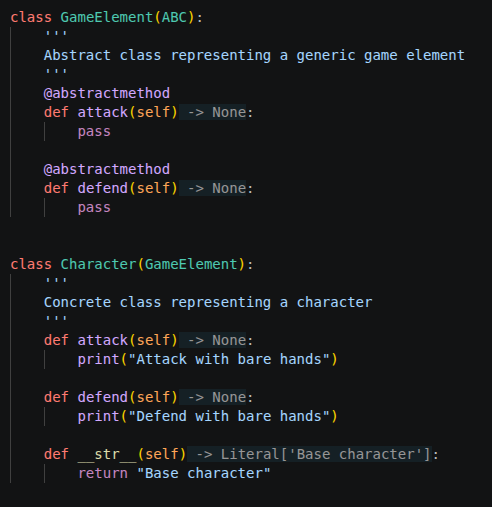
\includegraphics[width=0.3\textwidth]{1.png}
\end{center}

\begin{center}
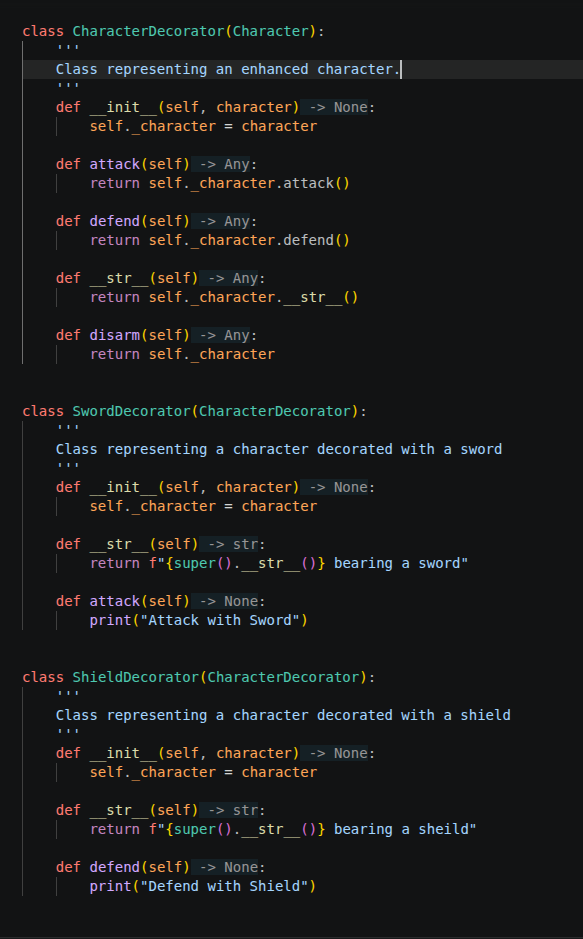
\includegraphics[width=0.3\textwidth]{2.png}
\end{center}

Needless to say, one cannot, and would never wish to, teach a large number of patterns. The number of distinct patterns taught is kept minimal (perhaps at most two or three patterns per category), focusing primarily on those patterns most commonly appearing in practice and that solve problems students are likely to have encountered in programming exercises during earlier course work. This approach was applied in an undergraduate software engineering course in a single lesson covering the topic of design patterns. That introductory lesson was subsequently followed by a practical application lesson that allows more open-ended problem solving activities. The course enrollment included students not only in the computer science major, but also in cyber science, systems engineering, and data science programs.
\section{Discussion}

What is the argument for a code-first approach?

If students first encounter a code example that solves a real problem, they can appreciate the motivation behind the pattern. When the abstract pattern is introduced afterward, it appears as a generalization of something they have already experienced rather than as an arbitrary diagram or UML structure.

Does that send mixed messages relative to other software development concepts?

Hands on practice with code. Examine the code, build and run it. What does it do?

Make a modification to it given instruction. This gets to the heart of what the design pattern is and does, i.e., what problem it is intended to solve.

Placement of lesson in the course.

Positioning of the course in the program curriculum.

Effectiveness.

To further place this work in context, we acknowledge Köppe's pitfalls related to the teaching of patterns~\cite{koppe2011}:
\begin{itemize}
\item Students often attempt to apply them too hastily
\item Insufficient experience to see design patterns' advantages
\item A tendency to overdo the application of patterns
\item Students do not necessarily see patterns as a best practice
\end{itemize}

\section{Conclusions and Future Work}

\begin{thebibliography}{9}

\bibitem{alahmad2006}
Al-Ahmad, W.,
\emph{Object-Oriented Design Patterns for Detailed Design}.
Journal of Object Technology 5:2, 2006.

\bibitem{carrington1998}
Carrington, D.,
\emph{Teaching Software Design and Testing},
Proceedings of the 28th Annual Frontiers in Education Conference (FIE '98), vol. 2, 1998.

\bibitem{carrington2018}
Carrington, D.,
\emph{What Can Software Engineering Students Learn from Studying Open Source Software?}.
International Journal of Engineering Education (IJEE) 24:4, 2018.

\bibitem{chimalakonda2018}
Chimalakonda, S., and Nori, K.,
\emph{A Patterns Based Approach for Design of Educational Technologies}.
Interactive Learning Environments 31:4, 2021.

\bibitem{gamma1994}
Gamma, E., Helm, R., Johnson, R., and Vlissides, J.
\emph{Design Patterns: Elements of Reusable Object-Oriented Software}.
Addison-Wesley, 1994.

\bibitem{gestwicki2008}
Gestwicki, P. and Sun, F.,
\emph{Teaching Design Patterns Through Computer Game Development}.
ACM Journal on Educational Resources in Computing (JERIC) 8:1, 2008.

\bibitem{hadar2008}
Hadar, I. and Leron, U.,
\emph{How Intuitive is Object-Oriented Design?}.
Communications of the ACM, 51:5 2008.

\bibitem{healy2023}
Healy, J.,
\emph{Game Design Learning: Understanding and Supporting the Game Design Process in Higher Education}.
Ph.D. dissertation, School of Media, Technological University Dublin, Dublin, Ireland, 2023.

\bibitem{koppe2011}
Köppe, C.
\emph{A Pattern Language for Teaching Design Patterns (Part 2)}.
Proceedings of the 18th Conference on Pattern Languages of Programs (PLoP '11), October, 2011.

\bibitem{lartigue2018}
Lartigue, J. and Chapman, R.
\emph{Comprehension and Application of Design Patterns by Novice Software Engineers},
Proceedings of the Annual ACM Southeast Conference, March, 2018.

\bibitem{nevison2003}
Nevison, C., and Wells, B., 
\emph{Teaching Objects Early and Design Patterns in Java Using Case Studies},
Proceedings of the 8th Annual Conference on Innovation and Technology in Computer Science Education (ITiCSE03), July, 2003.

\bibitem{pillay2010}
Pillay, N.,
\emph{Teaching Design Patterns},
Proceedings of the Southern African Computer Lecturers' Association Conference (SACLA), 2010.

\bibitem{schmidt1995}
Schmidt, D.,
\emph{Using Design Patterns to Develop Reusable Object-Oriented Communication Software}.
Communications of the ACM, 38:10, 1995.

\bibitem{sterkin2006}
Sterkin, A.,
\emph{Teaching Design Patterns}.
Proceedings of the Frontiers in Education: Computer Science and Computer Engineering Conference (FECS), 2006.

\bibitem{stuurman2004}
Stuurman, S., and Florijn, G.,
\emph{Experiences with Teaching Design Patterns}.
Proceedings of the 35th SIGCSE Technical Symposium on Computer Science Education (SIGCSE '04), March, 2004.

\bibitem{valdick2026}
Vahldick, A., and Vargas Nolli, J.,
\emph{Introducing the Visitor Design Pattern through a Digital Serious RPG Game}

\bibitem{wallingford1996}
Wallingford, E.
\emph{Toward a First Course Based on Object-Oriented Patterns}.
Proceedings of the 27th SIGCSE Technical Symposium on Computer Science Education (SIGCSE '96), March, 1996.

\bibitem{weiss2005}
Weiss, S.,
\emph{Teaching Design Patterns by Stealth}.
Proceedings of the 36th SIGCSE Technical Symposium on Computer Science Education (SIGCSE ’05), March, 2005.

\end{thebibliography}
\end{document}

